\section{Paul Traps}
It's safe to say that Paul traps have proven their worth as a valuable tool for working with trapped ions. Even outside of quantum computing, experiments involving trapped ions have provided crucial insight to many fields of physics over the last few decades. For us in particular, Paul traps utilizing RF electric fields and stationary qubit arrays are the focus of much research involving 2D Coulomb crystals. Given that importance, we'll take this opportunity to examine the theory behind Paul traps and how they may be implemented experimentally.

\subsection{Theoretical Framework}
Studying the work of Leibfried \textit{et al.}, we see a common model used to describe the electric potential $\Phi(x, y, z, t)$ of an RF trap \cite{Leibfried}. This assumes that the center of the trapping region has an approximately quadrupolar spatial shape, and that the function for the potential can be decomposed into a time-independent (static) part and a time-dependent part that depends on the RF drive frequency $\omega_{RF}$ such that
\begin{align}
    \Phi(x, y, z, t) &= U \frac{1}{2}(\alpha x^2 + \beta y^2 + \gamma z^2)\\ 
    \nonumber&+ {\widetilde{U}} cos(\omega_{RF}t) \frac{1}{2}(\alpha' x^2 + \beta' x^2 + \gamma' z^2).
\end{align}
Taking into consideration that this potential needs to satisfy Laplace's equation at all times, we get conditions for the geometric factors
\begin{align}
    &\alpha + \beta + \gamma = 0\\
    \nonumber &\alpha' + \beta' + \gamma' = 0.
\end{align}
There are multiple choices of appropriate values here that define various confining fields. Of interest to us is the choice
\begin{align}
    -(\alpha + \beta) &= \gamma > 0\\
    \nonumber \alpha' &= -\beta'
\end{align}
which dynamically confines particles in the $x$-$y$ plane and, at the same time, statically confines postively charged particles in the $z$-direction.

Ultimately, we want to understand the quantum mechanical interaction of ions trapped in RF fields (and we'll see that the quantized motion of trapped ions is closely approximated by static potential harmonic oscillators). Before we get to that point, we'll continue approaching the situation from a classical perspective.
\subsubsection{Classical Equations of Motion}
For simplicity, we'll consider motion only in the $x$-direction, but these equations are readily applied to motion in other directions. Using the potential in eq. (4), the motion of a particle with mass $m$ and charge $Z\abs{e}$ is given by
\begin{align}
    \ddot{x} &= -\frac{Z\abs{e}}{m} \partialderivative{\Phi}{x}\\
    \nonumber&= -\frac{Z\abs{e}}{m} \left[ U\alpha + \widetilde{U} \cos(\omega_{RF} t \alpha')\right] x
\end{align}
Using the substitutions
\begin{equation}
    \xi = \frac{\omega_{RF} t}{2}, \quad a_x = \frac{4Z\abs{e} U\alpha}{m \omega_{RF}^2}, \quad q_x = \frac{2 Z\abs{e} \widetilde{U}\alpha'}{m \omega_{RF}^2}
\end{equation}
we can rewrite Eq. (7) in the form of the Mathieu equation
\begin{equation}
    \derivative{^2 x}{\xi^2} + [a_x - 2q_x \cos(2\xi)] x = 0
\end{equation}
which is a known differential equation with periodic coefficients and having stable solutions that can be found with the Floquet theorem. 

For the sake of brevity, I'll leave out the complete derivation, but it suffices to say that the coefficients are recursively defined, and a numerical value must be extracted by truncating the continued fractions at the desired level of accuracy. The higher order contributions in the continued fraction typically fall off quickly for the values of $a_x$ and $q_x$ used in Paul traps.

What that work has done is allowed us to describe a region of stability in the potential field, and in particular, a lowest stability region---one which contains the point $(a_i, q_i) = (0,0), \quad \forall \: i \in \{x, y, z\}$. The actual shape of the stability region still depends on the geometric factors $\alpha$, $\beta$, and $\gamma$ which themselves depend on the applied RF field and trap electrodes (See Fig. )
\begin{figure}[h]
    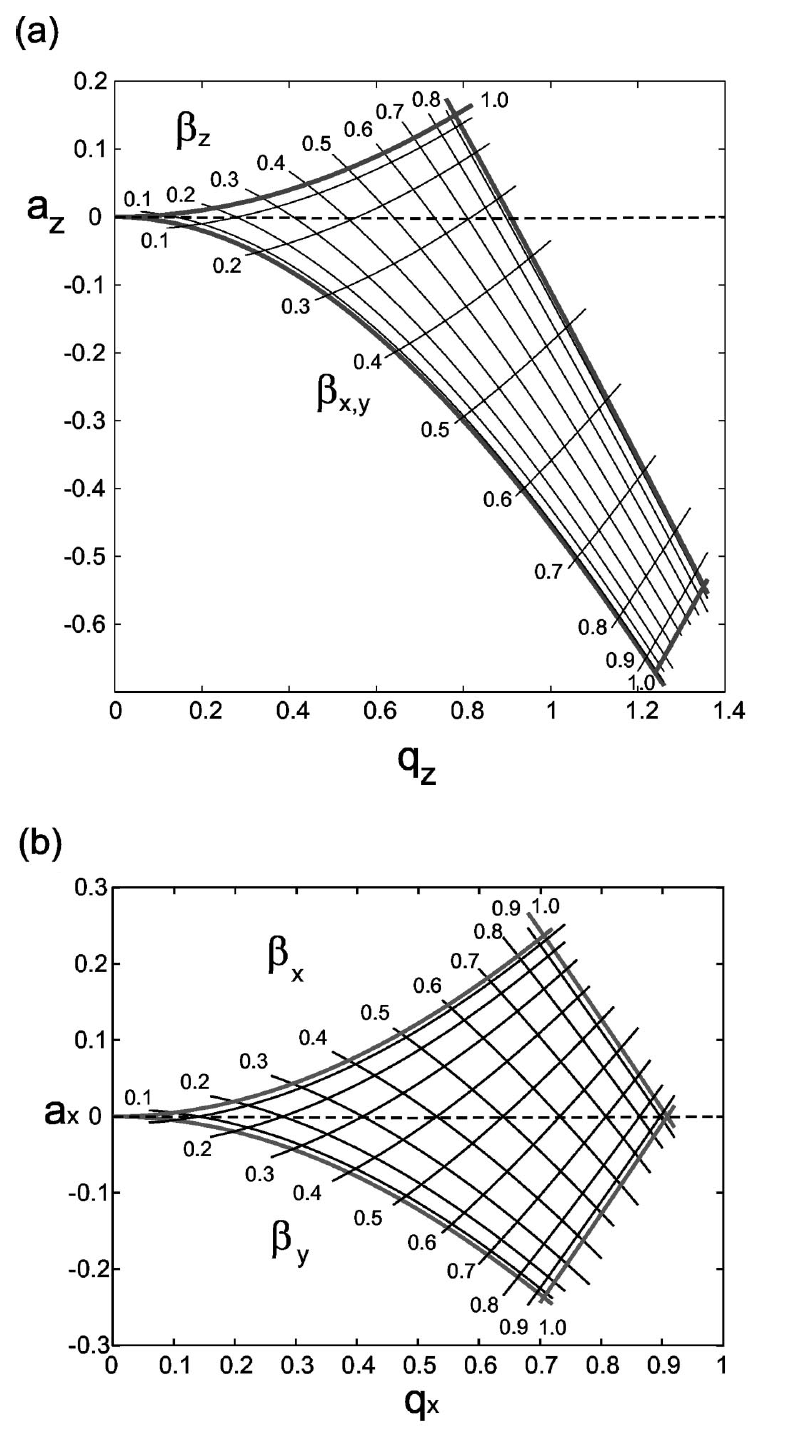
\includegraphics[width=\linewidth]{Leibfried - Stability Region.png}
    \caption{(\textbf{a}) yadda yadda}
    \label{fig:Stability Region}
\end{figure}


\subsection{Coulomb Interaction}
Run a manual sweep of anomalous airborne or electromagnetic readings. Radiation levels in our atmosphere have increased by 3,000 percent. Electromagnetic and subspace wave fronts approaching synchronization. What is the strength of the ship's deflector shields at maximum output? The wormhole's size and short period would make this a local phenomenon. Do you have sufficient data to compile a holographic simulation?

I have reset the sensors to scan for frequencies outside the usual range. By emitting harmonic vibrations to shatter the lattices. We will monitor and adjust the frequency of the resonators. He has this ability of instantly interpreting and extrapolating any verbal communication he hears. It may be due to the envelope over the structure, causing hydrogen-carbon helix patterns throughout. I'm comparing the molecular integrity of that bubble against our phasers.

We're acquainted with the wormhole phenomenon, but this... Is a remarkable piece of bio-electronic engineering by which I see much of the EM spectrum ranging from heat and infrared through radio waves, et cetera, and forgive me if I've said and listened to this a thousand times. This planet's interior heat provides an abundance of geothermal energy. We need to neutralize the homing signal.

Communication is not possible. The shuttle has no power. Using the gravitational pull of a star to slingshot back in time? We are going to Starbase Montgomery for Engineering consultations prompted by minor read-out anomalies. Probes have recorded unusual levels of geological activity in all five planetary systems. Assemble a team. Look at records of the Drema quadrant. Would these scans detect artificial transmissions as well as natural signals?

\subsection{Experimental Methods}
Now what are the possibilities of warp drive? Cmdr Riker's nervous system has been invaded by an unknown microorganism. The organisms fuse to the nerve, intertwining at the molecular level. That's why the transporter's biofilters couldn't extract it. The vertex waves show a K-complex corresponding to an REM state. The engineering section's critical. Destruction is imminent. Their robes contain ultritium, highly explosive, virtually undetectable by your transporter.

Communication is not possible. The shuttle has no power. Using the gravitational pull of a star to slingshot back in time? We are going to Starbase Montgomery for Engineering consultations prompted by minor read-out anomalies. Probes have recorded unusual levels of geological activity in all five planetary systems. Assemble a team. Look at records of the Drema quadrant. Would these scans detect artificial transmissions as well as natural signals?

\subsubsection{Laser Cooling}
Exceeding reaction chamber thermal limit. We have begun power-supply calibration. Force fields have been established on all turbo lifts and crawlways. Computer, run a level-two diagnostic on warp-drive systems. Antimatter containment positive. Warp drive within normal parameters. I read an ion trail characteristic of a freighter escape pod. The bomb had a molecular-decay detonator. Detecting some unusual fluctuations in subspace frequencies.

Sensors indicate no shuttle or other ships in this sector. According to coordinates, we have travelled 7,000 light years and are located near the system J-25. Tractor beam released, sir. Force field maintaining our hull integrity. Damage report? Sections 27, 28 and 29 on decks four, five and six destroyed. Without our shields, at this range it is probable a photon detonation could destroy the Enterprise.

Sensors indicate no shuttle or other ships in this sector. According to coordinates, we have travelled 7,000 light years and are located near the system J-25. Tractor beam released, sir. Force field maintaining our hull integrity. Damage report? Sections 27, 28 and 29 on decks four, five and six destroyed. Without our shields, at this range it is probable a photon detonation could destroy the Enterprise.

Communication is not possible. The shuttle has no power. Using the gravitational pull of a star to slingshot back in time? We are going to Starbase Montgomery for Engineering consultations prompted by minor read-out anomalies. Probes have recorded unusual levels of geological activity in all five planetary systems. Assemble a team. Look at records of the Drema quadrant. Would these scans detect artificial transmissions as well as natural signals?

It indicates a synchronic distortion in the areas emanating triolic waves. The cerebellum, the cerebral cortex, the brain stem,  the entire nervous system has been depleted of electrochemical energy. Any device like that would produce high levels of triolic waves. These walls have undergone some kind of selective molecular polarization. I haven't determined if our phaser energy can generate a stable field. We could alter the photons with phase discriminators.

\subsubsection{Radio-Frequency}
Communication is not possible. The shuttle has no power. Using the gravitational pull of a star to slingshot back in time? We are going to Starbase Montgomery for Engineering consultations prompted by minor read-out anomalies. Probes have recorded unusual levels of geological activity in all five planetary systems. Assemble a team. Look at records of the Drema quadrant. Would these scans detect artificial transmissions as well as natural signals?

We're acquainted with the wormhole phenomenon, but this... Is a remarkable piece of bio-electronic engineering by which I see much of the EM spectrum ranging from heat and infrared through radio waves, et cetera, and forgive me if I've said and listened to this a thousand times. This planet's interior heat provides an abundance of geothermal energy. We need to neutralize the homing signal.

Sensors indicate no shuttle or other ships in this sector. According to coordinates, we have travelled 7,000 light years and are located near the system J-25. Tractor beam released, sir. Force field maintaining our hull integrity. Damage report? Sections 27, 28 and 29 on decks four, five and six destroyed. Without our shields, at this range it is probable a photon detonation could destroy the Enterprise.

Communication is not possible. The shuttle has no power. Using the gravitational pull of a star to slingshot back in time? We are going to Starbase Montgomery for Engineering consultations prompted by minor read-out anomalies. Probes have recorded unusual levels of geological activity in all five planetary systems. Assemble a team. Look at records of the Drema quadrant. Would these scans detect artificial transmissions as well as natural signals?

\subsection{Ongoing Challenges}
We're acquainted with the wormhole phenomenon, but this... Is a remarkable piece of bio-electronic engineering by which I see much of the EM spectrum ranging from heat and infrared through radio waves, et cetera, and forgive me if I've said and listened to this a thousand times. This planet's interior heat provides an abundance of geothermal energy. We need to neutralize the homing signal.

Now what are the possibilities of warp drive? Cmdr Riker's nervous system has been invaded by an unknown microorganism. The organisms fuse to the nerve, intertwining at the molecular level. That's why the transporter's biofilters couldn't extract it. The vertex waves show a K-complex corresponding to an REM state. The engineering section's critical. Destruction is imminent. Their robes contain ultritium, highly explosive, virtually undetectable by your transporter.

\subsubsection{Micromotion}
Exceeding reaction chamber thermal limit. We have begun power-supply calibration. Force fields have been established on all turbo lifts and crawlways. Computer, run a level-two diagnostic on warp-drive systems. Antimatter containment positive. Warp drive within normal parameters. I read an ion trail characteristic of a freighter escape pod. The bomb had a molecular-decay detonator. Detecting some unusual fluctuations in subspace frequencies.

Sensors indicate human life forms 30 meters below the planet's surface. Stellar flares are increasing in magnitude and frequency. Set course for Rhomboid Dronegar 006, warp seven. There's no evidence of an advanced communication network. Total guidance system failure, with less than 24 hours' reserve power. Shield effectiveness has been reduced 12 percent. We have covered the area in a spherical pattern which a ship without warp drive could cross in the given time.

Shields up. I recommend we transfer power to phasers and arm the photon torpedoes. Something strange on the detector circuit. The weapons must have disrupted our communicators. You saw something as tasty as meat, but inorganically materialized out of patterns used by our transporters. Captain, the most elementary and valuable statement in science, the beginning of wisdom, is 'I do not know.' All transporters off.

Communication is not possible. The shuttle has no power. Using the gravitational pull of a star to slingshot back in time? We are going to Starbase Montgomery for Engineering consultations prompted by minor read-out anomalies. Probes have recorded unusual levels of geological activity in all five planetary systems. Assemble a team. Look at records of the Drema quadrant. Would these scans detect artificial transmissions as well as natural signals?

It indicates a synchronic distortion in the areas emanating triolic waves. The cerebellum, the cerebral cortex, the brain stem,  the entire nervous system has been depleted of electrochemical energy. Any device like that would produce high levels of triolic waves. These walls have undergone some kind of selective molecular polarization. I haven't determined if our phaser energy can generate a stable field. We could alter the photons with phase discriminators.

\subsubsection{Something Else}
Shields up. I recommend we transfer power to phasers and arm the photon torpedoes. Something strange on the detector circuit. The weapons must have disrupted our communicators. You saw something as tasty as meat, but inorganically materialized out of patterns used by our transporters. Captain, the most elementary and valuable statement in science, the beginning of wisdom, is 'I do not know.' All transporters off.

Deflector power at maximum. Energy discharge in six seconds. Warp reactor core primary coolant failure. Fluctuate phaser resonance frequencies. Resistance is futile. Recommend we adjust shield harmonics to the upper EM band when proceeding. These appear to be some kind of power-wave-guide conduits which allow them to work collectively as they perform ship functions. Increase deflector modulation to upper frequency band.

Run a manual sweep of anomalous airborne or electromagnetic readings. Radiation levels in our atmosphere have increased by 3,000 percent. Electromagnetic and subspace wave fronts approaching synchronization. What is the strength of the ship's deflector shields at maximum output? The wormhole's size and short period would make this a local phenomenon. Do you have sufficient data to compile a holographic simulation?

Sensors indicate human life forms 30 meters below the planet's surface. Stellar flares are increasing in magnitude and frequency. Set course for Rhomboid Dronegar 006, warp seven. There's no evidence of an advanced communication network. Total guidance system failure, with less than 24 hours' reserve power. Shield effectiveness has been reduced 12 percent. We have covered the area in a spherical pattern which a ship without warp drive could cross in the given time.

Now what are the possibilities of warp drive? Cmdr Riker's nervous system has been invaded by an unknown microorganism. The organisms fuse to the nerve, intertwining at the molecular level. That's why the transporter's biofilters couldn't extract it. The vertex waves show a K-complex corresponding to an REM state. The engineering section's critical. Destruction is imminent. Their robes contain ultritium, highly explosive, virtually undetectable by your transporter.